\section{Job Search with Correlated Wage Draws}
\begin{frame}{Deep look into the Policy Operator}
        $$
(T_\sigma v)(w) = \sigma(w) \frac{w}{1-\beta} + (1-\sigma(w))\left[c+\beta\textcolor{blue}{\underbrace{\int v(w')\, \varphi(dw')}_{\text{Dimension Reduction}}}\right]
$$
$$
\text{or equivalently, let $e(w):=\frac{w}{1-\beta}$}
$$

\begin{align*}
    T_\sigma v &= \underbrace{[\sigma e+(1-\sigma)c]}_{=:r_\sigma} + \underbrace{(1-\sigma)\beta \mathbb{E}v}_{=:K_\sigma v}\\
    &= r_\sigma + K_\sigma v
\end{align*}
\end{frame}

\begin{frame}{Comparison}
\textbf{For IID draws}
\begin{align*}
    T_\sigma v &= \underbrace{[\sigma e+(1-\sigma)c]}_{=:r_\sigma} + \textcolor{blue}{\underbrace{(1-\sigma)\beta \mathbb{E}v}_{=:K_\sigma v}}\\
    &= r_\sigma + \textcolor{blue}{K_\sigma v}
\end{align*}

\textbf{For Correlated wage draws}
\begin{align*}
    T_\sigma v &= \underbrace{[\sigma e+(1-\sigma)c]}_{=:r_\sigma} + \textcolor{blue}{\underbrace{(1-\sigma)\beta P}_{:=\beta P_\sigma}v}\\
    &= r_\sigma +\textcolor{blue}{\beta P_\sigma v}
\end{align*}
We assume $(W_t)$ is $P$-Markov with stationary distribution $\varphi$, $\int w\,\varphi(dw)<\infty$
\end{frame}

\begin{frame}{Optimality}
\begin{itemize}
    \item Value space is also Banach lattice
    \item $T_\sigma$ also order-preserving self-map
    \item Similar proof for well-posedness and regularity
    \item Similar affine and bounded by $\beta P$
    \item Same optimality results
\end{itemize}
    
\end{frame}

\begin{frame}{Difference}
\begin{itemize}
    \item wage draws are not iid anymore
    \item cannot reduce dimensions as before
\end{itemize}
    
\end{frame}
\begin{frame}{Reducing the value space}
    Let $\bar v:= (I-\beta P)^{-1}(e+c)$ and $V:= \{v\in L_1(\varphi): 0\le v\le \bar v\}$. Previously we have shown
    $$
    v_\sigma  = (I-\beta P_\sigma)^{-1}r_\sigma
    $$
    where $P_\sigma v =   (1-\sigma)P v \precsim Pv $, $r_\sigma  = \sigma e +(1-\sigma)c\precsim e+c$.\\
    \\
    
    Hence, we have
    $$
    v_\sigma \le \bar v
    $$
    By global stability and order preserving, $T_\sigma V\subset V$, i.e., self-map on $V$.
\end{frame}

\begin{frame}{Optimality on the reduced value space}
    \begin{figure}
        \centering
        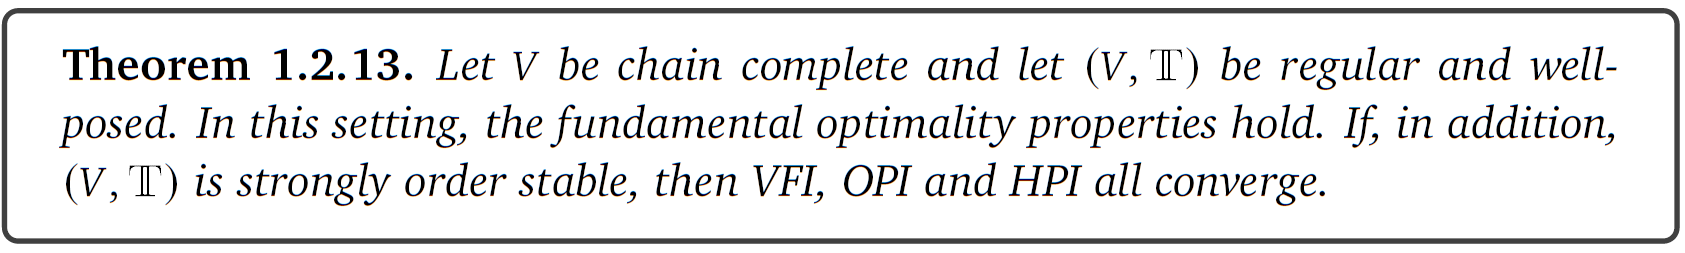
\includegraphics[width=1\linewidth]{Dynamic Programming/DP2/Chapter 4/Section 4.1.1. Job Search/thm 1.2.13.png}
        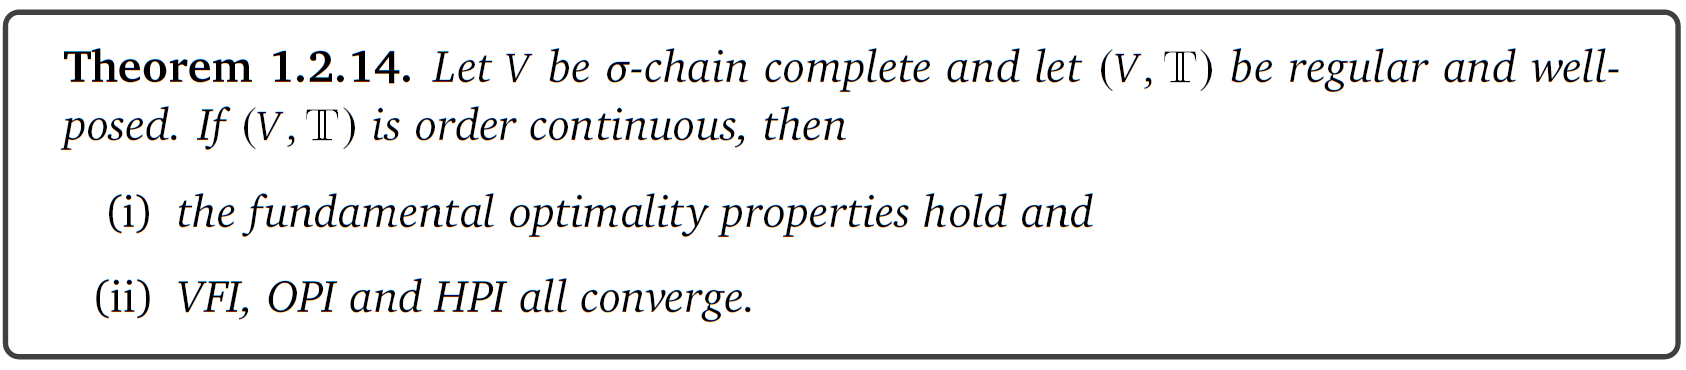
\includegraphics[width=1\linewidth]{Dynamic Programming/DP2/Chapter 4/Section 4.1.1. Job Search/thm1.2.14.png}
    \end{figure}
\end{frame}